%%%%%%%%%%%%%%%%%%%%%%%%%%%%%%%%%%%%%%%%%%%%%%
%% Template Thesis DGH UW v3.0
%%
%% Vincent Labatut 04/2015
%% Grégoire Lurton 07/2015
%%
%% v1   - 10/2014 : forme de rapport très différente
%% v2   - 02/2015 : modèle complètement refait
%% v2.1 - 03/2015 : définition de la page de titre
%% v2.2 - 03/2015 : correction de quelques bugs
%% v2.3 - 04/2015 : page de titre complétée (date, adresse postale, long titre)
%% v3.0 - 07/2015 : adaptation de la page de titre pour UW DGH
%% v3.1 - 07/2015 : inclusion de packages pour equations et test pour compilation knitr
%%%%%%%%%%%%%%%%%%%%%%%%%%%%%%%%%%%%%%%%%%%%%%
\documentclass[a4paper,11pt,draft,twoside]{article}

%%%%%%%%%%%%%%%%%%%%%%%%%%%%%%%%%%%%%%%%%%%%%%%%%%%
%% Loading Packages
%%%%%%%%%%%%%%%%%%%%%%%%%%%%%%%%%%%%%%%%%%%%%%%%%%%
\usepackage[english]{babel}
\usepackage[utf8]{inputenc}
\usepackage[T1]{fontenc}
\usepackage{mathpazo}
\usepackage{eulervm}
\usepackage[top=2.5cm, bottom=2.5cm, left=2.5cm, right=2.5cm]{geometry}
\usepackage{setspace}
\usepackage[colorlinks=true , final]{hyperref}
\usepackage[french]{varioref}
\usepackage{lastpage}
\usepackage{fancyhdr}
\usepackage[table]{xcolor}
\usepackage{lmodern}
\usepackage{amsmath,amsthm,amscd,amssymb}
\usepackage{eulervm}

\usepackage{tikz}
\usetikzlibrary{decorations.pathreplacing , chains , intersections}

\usepackage{pgfgantt}
\usepackage{pgfcalendar}





%%%%%%%%%%%%%%
\tikzset{
>=stealth',
  punktchain/.style={
    rectangle,
    rounded corners,
    % fill=black!10,
    draw=black, very thick,
    text width=10em,
    minimum height=3em,
    text centered,
    on chain},
  line/.style={draw, thick, <-},
  element/.style={
    tape,
    top color=white,
    bottom color=blue!50!black!60!,
    minimum width=8em,
    draw=blue!40!black!90, very thick,
    text width=10em,
    minimum height=3.5em,
    text centered,
    on chain},
  every join/.style={->, thick,shorten >=1pt},
  decoration={brace},
  tuborg/.style={decorate},
  tubnode/.style={midway, right=2pt},
}


%%%%%%%%%%%%%%%


\usepackage[numbers]{natbib}
\bibliographystyle{apa-good}

%%%%%%%%%%%%%%%%%%%%%%%%%%%%%%%%%%%%%%%%%%%%%%%%%%%
%% Paper's Information -- TO TWEAK
%%%%%%%%%%%%%%%%%%%%%%%%%%%%%%%%%%%%%%%%%%%%%%%%%%%
%TITLE
\newcommand{\reporttitle}{New approaches for the valorization of HMIS Data}

%AUTHORS
\newcommand{\reportauthors}{Grégoire Lurton}

%PROGRAM
\newcommand{\program}{PhD in Global Health}

%TRACK
\newcommand{\track}{Metrics Track}

%%%%%%%%%%%%%%%%%%%%%%%%%%%%%%%%%%%%%%%%%%%%%%%%%%%
%% Formatting stuff
%%%%%%%%%%%%%%%%%%%%%%%%%%%%%%%%%%%%%%%%%%%%%%%%%%%
\setlength{\headheight}{13.6pt} % due to a warning
\newcommand{\HRule}{\rule{\linewidth}{0.5mm}}
% Espace entre les paragraphes

% Headers and Footers
\pagestyle{fancy}
\fancyhf{}

\renewcommand{\headrulewidth}{0.4pt}
\renewcommand{\footrulewidth}{0.4pt}

\cfoot{\thepage}
\fancyhead[L]{\reporttitle}
\fancyhead[R]{\rightmark}

%%%% Define custom colors
\definecolor{grisclair}{rgb}{0.7,0.7,0.7}
\definecolor{grisfonce}{rgb}{0.5,0.5,0.5}
\definecolor{vert}{RGB}{74,171,67}

%%% PDF Metadatas
\hypersetup{
    pdftitle={\reporttitle},
    pdfauthor={\reportauthors},
    pdfsubject={\reporttitle},
    bookmarksnumbered=true,bookmarksopen=true,
	unicode=true,colorlinks=true,linktoc=all,
	linkcolor=blue,citecolor=blue,filecolor=blue,urlcolor=blue,
	pdfstartview=FitH
}

%%% Font  - Get sans serif
\renewcommand{\familydefault}{\sfdefault}


% Get Bulleted Lists Working
%\renewcommand{\FrenchLabelItem}{\textbullet}

%%%%%%%%%%%%%%%%%%%%%%%%%%%%%%%%%%%%%%%%%%%%%%%%%%
%%% WATERMARK

\usepackage{draftwatermark}
\SetWatermarkText{DRAFT}
%\SetWatermarkScale{5}



\begin{document}
%%%%%%%%%%%%%%%%%%%%%%%%%%%%%%%%%%%%%%%%%%%%%%%%%%%
%% Title Page
%%%%%%%%%%%%%%%%%%%%%%%%%%%%%%%%%%%%%%%%%%%%%%%%%%%
\phantomsection
\begin{titlepage}
	\begin{tikzpicture}[remember picture,overlay]
		\node at (current page.south west)
			{
            \begin{tikzpicture}[remember picture,overlay]
 				\pgftext[x=0cm,y=25.37cm,bottom,left]{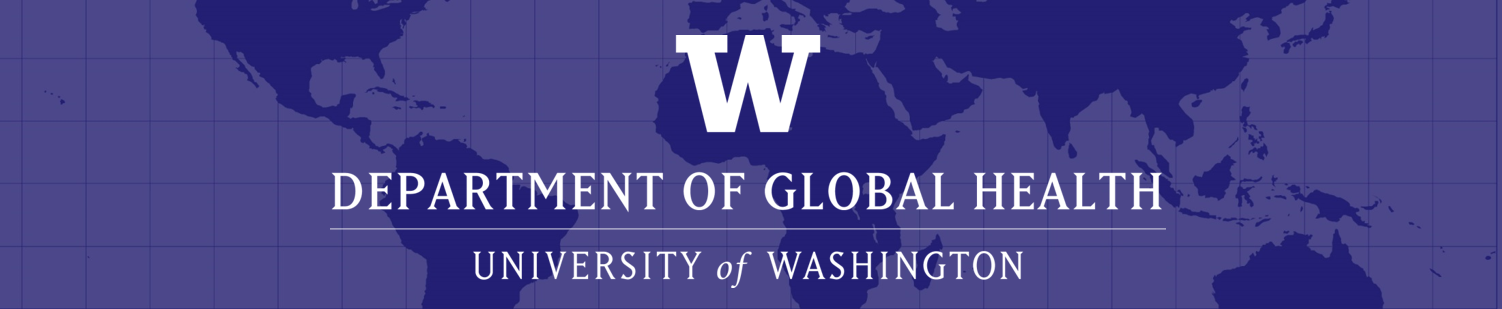
\includegraphics[width=21cm, draft = false]{images/dgh_banner.png}};
 				\pgftext[x=1.1cm,y=24cm,bottom,left]{\fontsize{20}{20}{\textbf{\program}}};
 				\pgftext[x=1.1cm,y=23.2cm,bottom,left]{\fontsize{18}{18}{\textbf{\textcolor{grisfonce}\track}}};
 				\pgftext[x=10.5cm,y=16.5cm,bottom,center]{\fontsize{30}{30}{\textbf{Methods and Issues for }}};%\reporttitle
                \pgftext[x=10.5cm,y=15.2cm,bottom,center]{\fontsize{30}{30}{\textbf{ the valorization of HMIS Data}}};
 				\pgftext[x=10.5cm,y=14.3cm,bottom,center]{\scalebox{0.77}[1]{\fontsize{20}{20}{\fontfamily{phv}\selectfont{}\textcolor{grisfonce}{\reportauthors}}}};
 				%\pgftext[x=5.5cm,y=13.1cm,bottom,left]{\scalebox{0.6}[1]{\fontsize{18}{18}{\fontfamily{phv}\selectfont{}\textbf{\today}}}};
 				\pgftext[x=1.1cm,y=1.8cm,bottom,left]{
\includegraphics[width=6cm , draft = false]{images/ihme_logo.png}};
                \pgftext[x=9.1cm,y=1.8cm,bottom,left]{
\includegraphics[width=6cm, draft = false]{images/itech_logo.png}};
                \pgftext[x=17.1cm,y=1.8cm,bottom,left]{
\includegraphics[width=3cm, draft = false]{images/bluesquare_logo.png}};
                \fill[fill=grisclair] (21cm,1cm) rectangle(0cm,0cm);
	\end{tikzpicture}
				};
			\end{tikzpicture}

\end{titlepage}

%% Get the page after title empty
\pagenumbering{gobble}% Remove page numbers (and reset to 1)
\newpage\null\thispagestyle{empty}\newpage


%%%%%%%%%%%%%%%%%%%%%%%%%%%%%%%%%%%%%%%%%%%%%%%%%%%%%%%%%%%%%%%%%%
%%%%    	FRONT MATTER
%%%%%%%%%%%%%%%%%%%%%%%%%%%%%%%%%%%%%%%%%%%%%%%%%%%%%%%%%%%%%%%%%%
\thispagestyle{plain}
\pagenumbering{roman}
\setcounter{page}{1}



\paragraph{Abstract}

Here the abstract will come

% Table des matières
\cleardoublepage
% Dans le cas du recto verso, ajoute une page blanche si besoin
\phantomsection
\tableofcontents
\addcontentsline{toc}{section}{Table of Content}
\newpage
\addcontentsline{toc}{section}{\listfigurename}
\listoffigures
\newpage
\addcontentsline{toc}{section}{\listtablename}
\listoftables

\thispagestyle{fancy}

% Justification moins stricte : des mots ne dépasseront pas des paragraphes
\sloppy

%%%%%%%%%%%%%%%%%%%%%%%%%%%%%%%%%%%%%%%%%%%%%%%%%%%
%%%% 	MAIN MATTER
%%%%%%%%%%%%%%%%%%%%%%%%%%%%%%%%%%%%%%%%%%%%%%%%%%%

%% Set page numbering right
\cleardoublepage
\pagenumbering{arabic}
\setcounter{page}{1}

\section{Introduction}

%% BIBLIO Shibuya05 "Health Statistics (...) are the basis for every aspects of health planning"
%% BIBLIO Shibuya05 Accountability stemming from MDGs
%% BIBLIO Shibuya05 WHO Dependent on data from countries that is usually bad quality #DataQuality
%% BIBLIO Shibuya05 Since 2003 WHO makes effort for better primary data collection #DataQuality
%% BIBLIO Nolen05 information essential to identify and understand health inequities


If a literary form had to be chosen to write or talk about Health Management Information Systems (HMIS), the complaint would probably be everyone's favorite pick. Be it complaints on the burden of work involved in collecting, managing and analyzing data in health systems, or laments on the inexistence of good quality data in most developing countries health systems, HIS are usually described as a non performing burdens of health systems, that can only be improved [HMN citation]. This frustration has multiple causes, and is only matched by the expectations placed in HIS and their widely recognized importance, some authors calling HIS "the foundation of public health"\cite{foundph}. Collecting and analyzing information on activities and results of health systems and on the populations served is indeed essential to guide strategic decision making and to inform health policies.

The complexity of designing and operating well performing national HMIS comes from the fact that HMIS have to handle a high diversity of data and information. Meanwhile, producing this information requires the contribution of a multitude of actors, and is a huge organizational and methodological challenge. Data used to produce relevant health information may come from administrative records, organizational documents or population surveys, and are produced by a variety of actors and organizations, with differing cultures and approaches.
% TODO lister les différents types d'info à produire.
% BIBLIO HMN Network
% BIBLIO walsh07 in IS in PVD issue, 3 / 4 papers are on health

Finally, HIS have to be able to adapt rapidly to changing epidemiological, organizational or political situations. They have to be able to produce relevant information on emerging health issues, and to adapt to the entry of new actors or to a modification in the mode of management of health systems.

In richer countries, the issue surrounding health information is often one of regulation and standardization. The  existence of well performing and well established data sources on populations, and the relative ease of collecting massive amounts of data on individuals pose questions that are mainly related to the protection of privacy, and to the definition of standards for interoperability. The definition of what information should or can be produced is usually a legislative and matter, handled by dedicated entities.

on est \gls*{who} et oui \gls*{who} plus \gls*{test}

%% BIBLIO Nolen05 Need to identify and understand inequities make it necessary to collect info on "specific health measures and equity stratifiers". #MoreData
%% BIBLIO Nolen05 Need to increase volume / diversify data collected. #MoreData #DataQuality

In developing countries, where population data is scarce and data collection can be much more of a challenge, the issues are much different. Health policies depend heavily on the financial, political and technical support of international actors, with differing orientations and priorities. As a consequence, developing countries HIS strengthening programs can be classified into two great families : technology based solutions and institutional reforms. The first family is mainly targeted towards improvement of data collection and relies on solutions relying on the revolution in  data collection capabilities. The second family relies on the adequation of health information produces to policy makers needs, and usually promotes a top-down and normative approach to Information Systems.

If each of these approaches has its benefits and some success stories,  they appear to miss an important part of what makes information systems work. They put their emphasis to the extremes of the information production chains (cf. Figure \ref{HMISFunctions}) and undervalue the middle tiers of these systems. This proposal designs research program oriented towards exploring ways in which this middle tier can be mobilized to improve the value of information produced by HMIS.

This document will start by an introduction of the conceptual framework surrounding the proposed research. We will define Health Management Information Systems, using two classic schematic approaches. We will then define the objectives we will pursue in our research, and will finally describe our different aims and the methods we want to use to complete them.


\newpage
\section{Conceptual framework}

There is a lot of talk about how a data revolution could improve the management of governements in developing countries, and how it could help 

In order to strengthen Health Information Systems, one needs to understand their political logic and traditions. Working with HIS professionals, one clear perspective is the confusion in one HIS are or are not, what they are supposed to achieve and how they are supposed to do it. The confusion in a lot of official documents between health information and Monitoring and Evaluation is a sign of this blur between concepts and approaches.

As such, information systems are complex political and technical projects, with histories, traditions and perspectives. In former colonies, these histories and traditions have been, at least in part, inherited from the former colonial traditions, and in countries in which foreign aid is an important composant of health systems, new concepts and ideas are still introduced. What is the coherence of these systems, once all these traditions have been digested ? How can coherent systems emerge from these melting pots of ideas and

It is essential that actors that interest themselves in the development and strengthening of health information systems in developing countries be aware, and understand these tensions, to offer solutions that make sense and are productive.

As complex objects, most actors have a very partial and parcellar understanding of what they do and what they are.

The way in which health information systems are represented have evolved over time, as technical conditions of their existence was also evolving. From an ad-hoc and centralized vision of simple tallies in the XIXth century %need citation
to complex organisational and technological systems in the latest iterations. To justify our approach, we will first consider the evolution of these representations, and derive an approach that will build on the latest evolutions.

In sub-Saharan Africa, the way health information systems have evolved is heavily influenced by both medical traditions of colonizing powers, and their statistical traditions.

Historian of statistical thought Alain Desrosières describes a succession of stages in the development of public statistics.

It does not really make sense to trace the development of health information system in sub-saharan Africa to times anterior to colonial times. The production of data on colonial empires was primarily focused on the production of

\subsection{Two domains}

There are two main domains of health information systems. One is interested with the description of the populations and the health related events that they suffer, and the other is interested in the description and understanding of health services for this population. These two domains are using inherently different data sources %citeHMN.
and answer to different logics. Population based data sources come from the tradition and use the techniques developped by social statisticians, using sampling based data methods, or purely administrative records for censues. Health services data comes from a more recent tradition, and have developed in a managerial approach. Here, different traditions have given different objectives to faciltiies based statistics. The english tradition, pioneered by Florence Nightingale and Carr , have focused on the evaluation of mortality, and a very early focus on evaluation of quality of care. Meanwhile, the french approach was much more focused on the administrative use of this data, and early facilities registers are purely counts of cases and beneficiaries, for police and administrative purposes.


\subsection{Early days}

\subsection{Managerial Approach}

%% BIBLIO HMN Framework

\subsubsection{Goal approach}
\label{sec_goal}


A first approach to HMIS is a consideration of the stated goals of these information systems. Figure \ref{HMISGoals} shows what these main goals are.
\begin{figure}[htp]
	\centering
	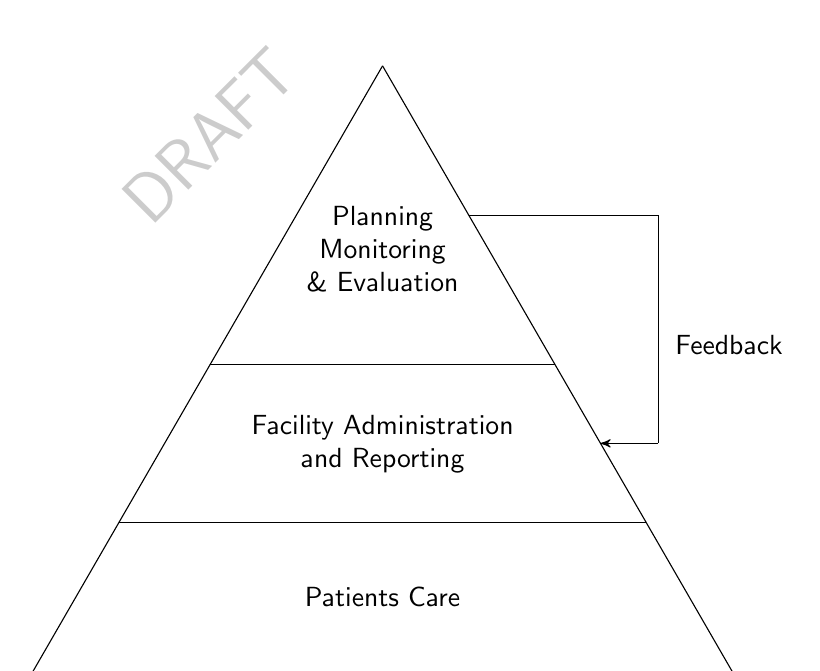
\begin{tikzpicture}[node distance=2cm]
		\coordinate (A) at (-4.5,0) {};
		\coordinate (B) at ( 4.5,0) {};
		\coordinate (C) at ( 0,7.7942) {};
		\draw[name path=AC] (A) -- (C);
		\draw[name path=BC] (B) -- (C);
		\draw (1.1,5.8971)--(3.5,5.8971) ;
		\draw(3.5,5.8971)--(3.5,3) ;
		\draw [->](3.5,3)--(2.77,3) ;
		\node at (4.4,4.25) {Feedback};
		\foreach \y/\A/\txtHigh in {0/Patients Care/0.8 ,2/Facility Administration \\ and Reporting/2.5,4/Planning \\ Monitoring \\ \& Evaluation /4.8}{
			\path[name path=horiz] (A|-0,\y) -- (B|-0,\y);
			\draw[name intersections={of=AC and horiz,by=P},
			name intersections={of=BC and horiz,by=Q}] (P) -- (Q)
			node[align = center,above] at (0,\txtHigh){\A};
		}
	\end{tikzpicture}
	\caption{Information needs for HMIS}
	\label{HMISGoals}
\end{figure}

\begin{description}
	\item[Patients Care] Taking care of patients is the primary goal of a health facility. To do so, it is necessary to collect data on these patient, data that will be transmitted (to other services), stored and reused during further follow-ups.
	%BIBLIO chaperon88 medical most important et doit diriger le reste
	\item[Facility Administration and Reporting] At facility level, HMIS data is used in daily activities to quantify and forecast needs in health inputs, and to create reports for higher levels of the health system. @spiegel
	\item[Planning, Monitoring \& Evaluation] People in charge of the administration of health systems at local or national also need data to monitor activities in the health system, to evaluate the results of interventions, to report to funders or to plan later interventions.
\end{description}

The pyramidal representation of these needs is used to show that these goals fill data needs at different levels of health systems. The different needs for information can roughly thought as being the needs of different type of actors of the health system. Meanwhile, this understanding is not fully true, as at local level, actors will often hold multiple roles and will thus have to use information in different situations. For example, a physician may also be in charge of managing his health facility, and will thus need to plan activities and report on them.



\subsubsection{Functional approach}
\label{sec_function}

A first way to approach HMIS is to describe the four principal functions that are necessary to have a HMIS to run. Figure \ref{HMISFunctions} presents a simplified sketch of the principal functions that are to be filled in order for HMIS to produce useful information.

\begin{figure}[h]
	\begin{center}
		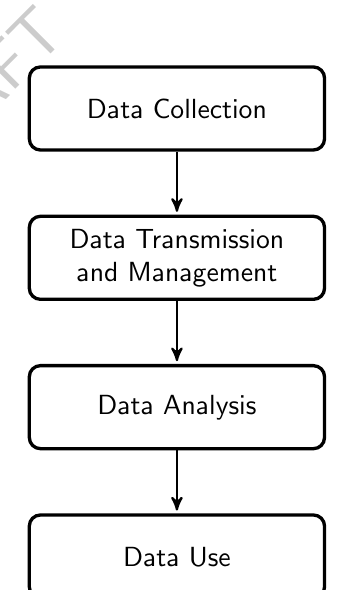
\begin{tikzpicture}[node distance=.8cm,  start chain=going below,]
			\node[punktchain, join] (DataCollection) {Data Collection};
			\node[punktchain, join] (DataManagement) {Data Transmission and Management};
			\node[punktchain, join] (DataAnalysis)   {Data Analysis};
			\node[punktchain, join] (DataUse) 		  {Data Use};
		\end{tikzpicture}
	\end{center}
	\caption{Different functions inside the Health Information Systems}
	\label{HMISFunctions}
\end{figure}

\begin{description}
	\item[Data Collection] Primary data collection is essential to the production of any information system. In the case of HMIS, data collection happens in health facilities, and is made by health professionals. Data collected in health facilities can be individual patient data collected in patients files or cards. It can also be a first level of aggregation of this data, as for indicators that are reported on a regular basis by facilities to higher levels of the health system. This reporting usually happens through standardized reports, that are then transmitted by successive aggregation to the top of the health pyramid.

	\item[Data Management] Data collected in health facilities has to be stored and archived, to be later accessed and reused. Data management work can encompass managing paper data, or managing computerized data. Individual patient data will be computerized in \gls*{emr} whereas aggregated indicators are stored in data-warehouses, like the DHIS2 software.

	\item[Data Analysis] Data that is collected and stored in HMIS can then be analyzed. Analysis can be defined as the transformation of data into information. The results of data analysis can be varied, from collection of graphs and maps that can constitute dashboards, to the results of complex models that provide evidences of causality.

	\item[Data Usage] Information is the end product of the HMIS, and is used by decision makers or health workers to achieve their tasks. For example, a nurse in a health post may need the monthly consumption of a health product to place an order. A District Health Officer may consider the evolution of monthly number of cases of malaria in his district to plan malaria prevention activities. At national level, a worker at the Ministry of Health may use the number of patients tested positive for HIV to design grant applications for the Global Fund.
\end{description}

Even though the schematic representation of this functions is linear, it should be noted that this linearity is not true in practice. Even once data has been analyzed the results of this analysis has to be archived, and transmitted to the information end users. In some situations, data can be used in its raw form. For example, a physician may use a biological result that he has received in a raw form. Finally, for some data, data collection won't happen inside the health  facility. For example, population survey results may be used to plan and target some interventions, but primary data collection will have happened outside of the health system, and the first function to be used in the HMIS will be the data management function.

The way a program considers and plans each of these functions will define how a specific HMIS will work. We will now present three common approaches to HMIS.



\subsection{Era of Big Data}

%OpenHIE

\subsection{A typology of HIS approaches}

Based on this historical, we tend to describe different approaches to HMIS in developing countries, and different approaches and to present a typology of strengthening strategies.

\subsubsection{Three HMIS archetypes}

Functions of HMIS (cf. section \ref{sec_function}) are not independent of each other. Defining the relative importance of different functions of HMIS in the overall systems can change greatly the way a HMIS functions, and the output it produces. We differentiate three paradigmatic types of HMIS, varying on the respective influence of different functions. Building on the idea that a HMIS is used to provide an image of the activities and performances of a health system, we describe each function as a different way of making an image.

\paragraph{Jigsaw Puzzle HMIS} - A common way to design HMIS in developing countries can be considered as a Jigsaw Puzzle approach. A series of indicators are designed by program managers. These indicators are deemed to be \textit{sensitive} and \textit{specific}, and are supposed to allow managers to track and identify precisely the performance of health systems, and to provide important information on health system's results. The HMIS will then be organized to produce carefully designed indicators at facility level, and to transmit these indicators to higher levels for aggregation.

In these types of system, a lot of importance given to data collection functions, as the quality of this primary data collection is key to the rest of the work in the system. Data management in these system is often limited to aggregating some data and transmitting it to different actors in the health systems. Data analysis is usually mainly descriptive and is limited to presentation of time series values or mapping of indicators along administrative boundaries.

These systems are similar to jigsaw puzzles, made of specific pieces, to compose a predetermined picture. When they are well designed, these systems can provide useful information on health systems. Meanwhile, they are vulnerable to any variation in primary data collection. As for jigsaw puzzles having a piece missing will jeopardize the possibility to get the whole picture right.

\paragraph{Pixel HMIS} - Another way to conceive HMIS is built on the collection and use of a multitude of individual data collected through  \gls*{emr}. Once the data is collected, program managers can query different indicators on different levels of aggregation, that can be extracted from different EMRs. In the best situations, interoperability of multiple  \gls*{emr} present in a country allow for a central analysis of the data \cite{pugliese2009large}.

These systems allow a great variety of analysis, with a great variety of approaches. Analysis can be led varying geographic and time focus, or changing definitions of computed quantities. It also allows longitudinal analysis that are more difficult to perform with other approaches.

This approach thus involves a great investment in primary data collection and management, and allows elaborate data analysis. Meanwhile, it requires a technological investment and maturity that is seldom achieved in rich countries, and thus is very rare in developing countries.

\paragraph{Tangram HMIS} - Between the two extremes that are puzzle and pixel HMIS is a third, less prevalent approach to HMIS. This approach will be compared to the tangram game, in which simple forms are used and reused to draw different pictures. In this approach, the emphasis is put on the management functions of HMIS. Simple data elements are collected and stored, and are used and combined in different ways depending on the analysis that is done.

A key component of this model is thus the ability to store and reuse data, thus putting an emphasis on the middle tiers of data management. The use of data warehouses for computerized data is thus a characteristic of this approach. Meanwhile, it also requires an emphasis on data analysis in order to provide relevant information to end users.

\subsection{HMIS strengthening strategies}

Depending on the HMIS model that is used, programs will implement different type of HMIS strengthening approaches. Programs who privilegy a jigsaw puzzle approach to HMIS will tend to focus on standardizing procedures and methods for data collection and data analysis. Meanwhile, programs who privilegy a pixel approach to HMIS will tend to favor solutions geared towards the implementation of new and performing data collection tools.

\begin{description}
	\item[The institutional approach] operates under the assumption that all functions of information systems should be geared towards and submitted to the end information users. This approach tends to be extremely normative as any activity in the information system has to be oriented towards one main predefined goal. In doing so, this approach undervalues the benefits of both the integration of external data, and the positive externalities data collection and analysis may have on multiple users.

	% BIBLIO thieren05 besoin d'harmonisation #InstitutionalApproach
	% BIBLIO chaperon88 1958 reform of hospital morbidity collection forms from methods at Hotel Dieu : elle va tres rapidement echouert: le questionnaire demande un sercroît de travail aux services administratifs confrontés dans le même temps à une nomrlasation de l'ensemble des imprimiés : côté médical l'investigation est ressentie comme un contrôle de l'administration sur l'activité médicale. (FROM RAZPPORT ECOLE DES MINES)
	% Tradition française : médical prime...

	% BIBLIO braa07 "the top-down and all-inclusive approach to standardization common among ministries and central agencies"
	% BIBLIO braa07 "the individual standards must be crafted in a manner which allows the whole complex system of standards to be adaptive to the local context"
	% BIBLIO braa07 principle of flexible standards, and the principle of integrated independence.
	% BIBLIO braa07 we can get rich infor- mation from minimal data. A focus on the must-know rather than nice-to-know information, as illustrated by the emphasis on indicators and the minimal essential data set, can be extremely powerful in that it allows a simple, well-chosen data element to be used for several purposes.
	% BIBLIO braa07 Second, accept that there will always be technically incompatible subsystems.

	\item[The technological approach] relies on the assumption that collecting data and making it available is a sufficient enabler for all other functions of information systems to operate. In this sense, a direct link is made between an information need and a data gap. This approach comes at a cost, and provides only limited benefits if it is not supported by improved data analysis. These solutions tend to provide highly specialized and siloed data collection systems.
	% CITE macfar05 "The availability of powerful computers and of reasonably priced software has led to a proliferation of database systems" #ICTBased

\end{description}

We argue these two approaches focus on the most expensive ways to strengthening HMIS (data collection and systemic reforms), and are emphasizing the design of systems and tools that are specific to precisely defined data needs, thus limiting the possibility to implement secondary data usage and the positive externalities of their interventions. The archetype of these pitfalls are the well known parallel and siloed data systems present in many developing countries health systems.

Meanwhile, some of the most significant successes in the strengthening of health information systems in developing countries have been reached precisely through the strengthening of their middle tier. The District Health Information System (DHIS2) project has become a pervasive system to store and organize data collected in developing countries health systems. The DHIS2 approach to health information is based on the organization and storage of multiple data types and sources in a generic data warehousing approach. Its versatility and its ability to adapt to different contexts and data has made it increasingly used in multiple context, thus arguably improving the storage and the availability of health data in low resources countries. Other approaches geared towards the promotion of interoperability of different dimensions of data systems, such as the Open Health Information Exchange framework are also gaining traction.

% CITE OHIE

If these approach have provided efficient solutions to organize and access HMIS data, there is still a lack of solutions to analyze and use HMIS data. Indeed, the high dimensionality of HMIS data and its average low quality make it essentially hard to analyze using standard methods available in developing countries health systems. We will now describe the research project developed to explore ways to analyze this data.

We want to ancher hospital data in a multiplicity of data sources that are available to health professionals to create evidence and make decisions. This data can be metadata that is routinely generated during data collection exercises. It can also be data generated by other organisations of the community. Finally, it can be similar data generated by different actors.

We will explore and propose ways to use these different types of data. First, we will


\subsection{Approach and research questions}

% BIBLIO walsh07 Structuration des questions IS in dvt countries in 4 dimensions : #ICTBased
%% 1. Link ICT and Development
%% 2. Cross cultural aspect of ICT
%% 3. Local Adaptation
%% 4. Marginalized groups



This project aims at exploring methods to improve the analysis and use of HMIS data by providing innovative approaches to this data. To do this, we will use both a technical approach using innovative methods from the data science field, and a critical approach of health information systems as social objects.

The generic question we ask is : How can data currently routinely used data sources be used to provide actionable information for decision makers ?

More precisely, we will ask three main data analysis questions :
\begin{itemize}
	\item How can metadata collected in an EMR be used in EMR data analysis ?
	\item How can different non standardized HMIS sources be mapped and jointly analyzed ?
	\item How can multiple data source be integrated to HMIS and analyzed to provide information at local level ?
	\item How do decision makers in health systems consider HMIS generated data, and how does it influence the way HMIS are engineered ?
\end{itemize}

% BIBLIO macfar05 : Type d'organisation HMIS depend de culture locale et type d'organisation statistique nationale
% BIBLIO macfar05 : Difficultés pour faire système statistique local :
%% 1. diversité des sources
%% 2. Local data needs vs central
%% 3. Harmonization vs disaggregation
%% 4. Health Resource
%% 5. Confidentiality
%% 6. Incentives
% BIBLIO macfar05  Technology "The Availability of powerful computers and of reasonably priced software has led to a proliferation of database systems"  #SolutionType

%BIBLIO chaperon88 la nécessité d'une conception souple, non exhaustive et évolutive de tels systèmes privilégiant les indicateurs multiples adaptés aux différents niveaux de responabilité et aux différents objectifs #NormeFaible

list projects

Categorize through type of data and methods used.

%TODO vision unifiée sur outillage statistique => Approche bayesienne
%TODO on considere que progres dans HMIS ne peut pas venir d'un progres dans une seule dimension. On fait donc un projet sur tous les tableaux en meme temps

%%%%%%%%%%%%%%%%%%%%%%%%%%%%%%%%%%%%%%%%%%%%%%%%%%%%
Our method is taken in a decision theoretic framework. We do not aim at providing substantial knowledge with the results of our analysis, but rather we aim at providing information that will emopower decision makers to take decisions.

Cadre bayésien %%BIBLIO SPIEG04 Decision theoretic framework.
%% CITE SPIEG04 "Since advances in health-care typically happen through incremental gains in knowledge rather paradigm-shifting breakthroughs, this domain appears particularly amenable to a Bayesian perspective."

We operate in decision theoretic framework, our end objective being to inform decision making for the

Approche Probabilistique des données

Control Charts
%%%%%%%%%%%%%%%%%%%%%%%%%%%%%%%%%%%%%%%%%%%%%%%%%%%%



Each of these questions explores a different aspect of how standard HMIS data analysis can be expanded to produce useful information with HMIS data. Metadata like the times of creation and savings of EMR forms are indeed seldom used. Meanwhile they provide useful information on how data is collected, and on the working patterns inside health facilities. Our second question explore a different problem, which is often taken as a question of interoperability. Indeed the multiplicity of programs and actors working in many health systems generates a multiplicity of indicators used, that are often related but not identical. There is a need for simple and effective methods to map and conjointly analyze data from different HMIS systems. Finally, HMIS should be useful for local level analysis and decision making. Meanwhile, HMIS data is seldom useful on its own and has to be integrated in larger analysis frameworks to produce interesting information. This integrating can be difficult at national level, but it is even more complicated at local levels, has mapping precisely different data becomes more and more of a challenge at small scale.

We also aim at providing a critical evaluation of the way HMIS are thought of in developing countries societies. Authors like Alain Desrosières and Ted Porter have shown how statistics and computation have come from and generated different cultures of public action in modern societies. The ambivalence of numbers as descriptors or norms has an influence on how information systems are thought of as top-down normative systems instead of knowledge systems. We aim at interrogating how this perception has its roots in long term local historical trends as well as in the tradition and methods of quantitative public health.


To answer these question, we will conduct four distinct research projects.
\begin{description}
	\item[Aim 1] Evaluation of the benefits of improved data collection for HIV patient care in Kenya.
	\item[Aim 2] Test of multiple semantic approaches to interoperability in Bénin.
	\item[Aim 3] Definition and test of a local malaria elimination metric in Namibia.
	\item[Aim 4] Analyze of the theory and practices of Health Information Systems for national decision makers in Mali.
\end{description}

These aims have been designed to provide insights on the problematic posed for each HMIS goal and function. We will now describe each of these aims in more details.


\newpage
\section[EMR and individual health]{EMR and individual health\footnote{This section is heavily based on KenyaEMR evaluation protocol.}}

A first aim will be to understand how data collection itself impacts quality of care. As we postulate that data collection is not a neutral activity, we want to look into how primary data collected in HIV care setting can impact the outcome of care and organizational capabilities of HIV services. The case we will explore for this project is provided through a project implemented by ITECH in Kenya.

\begin{figure}[ht]
\begin{minipage}{.4\textwidth}
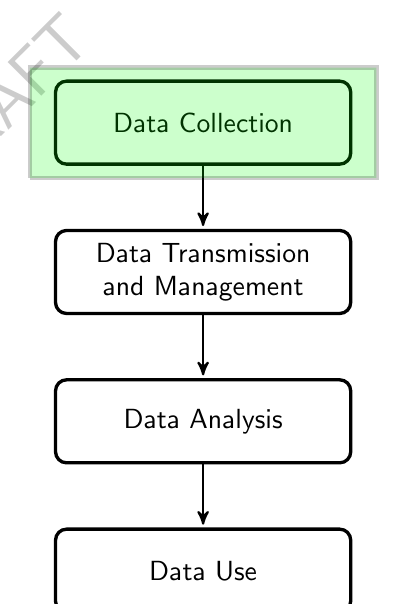
\begin{tikzpicture}[node distance=.8cm,  start chain=going below,]
     \node[punktchain, join] (DataCollection) {Data Collection};
     \node[punktchain, join] (DataManagement) {Data Transmission and Management};
     \node[punktchain, join] (DataAnalysis)   {Data Analysis};
     \node[punktchain, join] (DataUse) 		  {Data Use};
     \filldraw[ultra thick, draw=black, fill=green, opacity=0.2] (-2.2,-.7) -- (-2.2,.7) -- (2.2,.7) -- (2.2,-.7) -- (-2.2,-.7) ;
\end{tikzpicture}
\end{minipage}
\begin{minipage}{.5\textwidth}
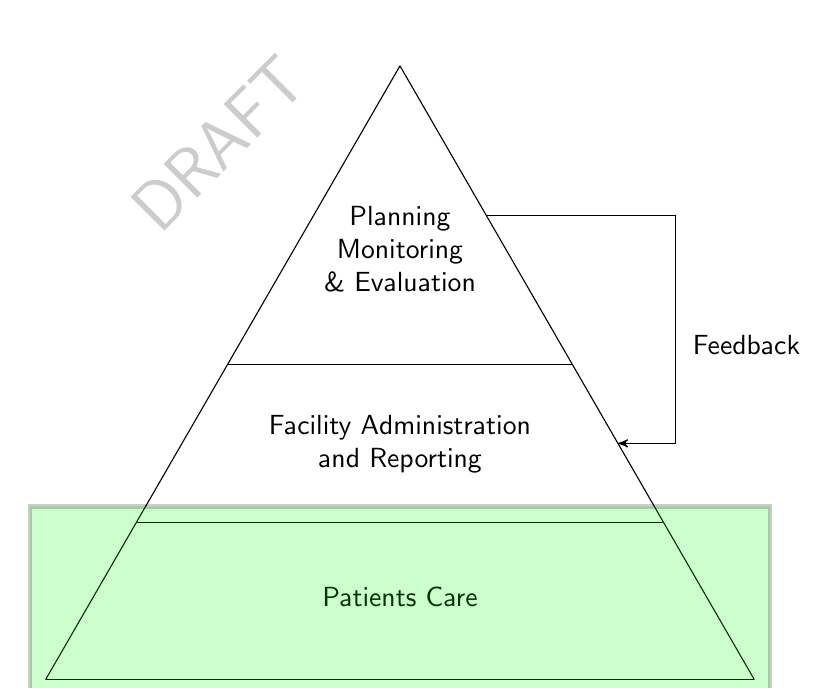
\begin{tikzpicture}[node distance=2cm]
\coordinate (A) at (-4.5,0) {};
\coordinate (B) at ( 4.5,0) {};
\coordinate (C) at ( 0,7.7942) {};
\draw[name path=AC] (A) -- (C);
\draw[name path=BC] (B) -- (C);
\draw (1.1,5.8971)--(3.5,5.8971) ;
\draw(3.5,5.8971)--(3.5,3) ;
\draw [->](3.5,3)--(2.77,3) ;
\node at (4.4,4.25) {Feedback};
\foreach \y/\A/\txtHigh in {0/Patients Care/0.8 ,2/Facility Administration \\ and Reporting/2.5,4/Planning \\ Monitoring \\ \& Evaluation /4.8}{
    \path[name path=horiz] (A|-0,\y) -- (B|-0,\y);
    \draw[name intersections={of=AC and horiz,by=P},
          name intersections={of=BC and horiz,by=Q}] (P) -- (Q)
          node[align = center,above] at (0,\txtHigh){\A};
          }
    \filldraw[ultra thick, draw=black, fill=green, opacity=0.2] (-4.7,-.2) -- (-4.7,2.2) -- (4.7,2.2) -- (4.7,-.2) -- (-4.7,-.2) ;
\end{tikzpicture}
\end{minipage}
\caption{Objective one definition}
\label{Paper One}
\end{figure}


    \subsection{Setting}

In Kenya, I-TECH has implemented an EMR for HIV care, called KenyaEMR, in 341 facilities. The evaluation of this program is currently being carried out. One objective of this evaluation is to assess the effectiveness of KenyaEMR implementation. This effectiveness will be evaluated on two dimensions:

\begin{enumerate}
\item	Improvement of reporting quality in facilities after KenyaEMR implementation
\item	Improvement of quality of care metrics after KenyaEMR implementation
\end{enumerate}

    \subsection{Data}

Kenya’s legal framework for protection of confidentiality of personal health information prohibit transfer of individual patient-level data from any health care facility, even if the data is de-identified. For this reason, the data we will use for this evaluation will be indicators of quality of care, aggregated monthly at facility level, and used for Continuous Quality Improvement (CQI) (see section \ref{sec:qual_of_care}). These indicators will be aggregated on site in Kenya and transmitted for data analysis.

To monitor the maturity of implementation of KenyaEMR (see section \ref{sec:maturity}), we will measure the delay in data entry using metadata stored with KenyaEMR forms, with time stamps for form creation. We will also trace utilization of reporting features of KenyaEMR by using time stamps linked to the use of reports generation. All this data will be extracted and transmitted in raw form for analysis.

To measure the quality of the reports produced for different periods (see section \ref{sec:rep_quality}), we will consider counts of number of forms entered for a given period, and mean completeness of entered forms. These will be aggregated on site and transmitted for data analysis. We will also use results from Routine Data Quality Assessments (RDQA) that have been conducted in different sites with KenyaEMR implementation. Data for these RDQA are collected in Excel format, and will be used as an external measure of the quality of data entered in KenyaEMR.
In the remaining of this document, we will thus use the following terms:
\begin{itemize}
\item Patient data refers to the data collected by health workers during patients’ visits. They are stored in paper patients’ files, or entered in KenyaEMR forms. We will thus refer to paper patient data or to electronic patient data. This data will not be directly used for analysis in this project.
\item CQI indicators refers to aggregated indicators used to measure quality of care.
\item CQI Report refers to a set of CQI indicators computed for a specific month for a specific facility.
\item DHIS Report refers to the MOH 731 and MOH 711 reports. We will differentiate between paper reports for which the data and the computation of indicators have been made without any digitalization of patients’ data, and electronic reports for which patients’ data has been digitalized. We will be able to use the paper reports as they have been entered in DHIS2 or other data collected by health districts administrations.
\item Patient Forms Metadata refers to the metadata generated by KenyaEMR when patient forms are entered. The metadata used should mainly be timestamps related to time of data entry.
\item Reporting Metadata refers to timestamps generated by KenyaEMR when different types of report are generated.
\item RDQA Data refers to raw data collected during RDQA exercises.
\end{itemize}

    \subsection{Implementation maturity}
    \label{sec:maturity}

We distinguish three different periods in the implementation of the EMR. Each of these periods is characterized by different ways the data is collected, entered, analyzed or used. For each of these periods, we will also have access to different types of data. We will describe the characteristics of each of these periods, and present a strategy to categorize the available data in each of these periods, using DHIS and CQI reports and metadata.

        \subsubsection{Paper Based}

In the first period, no patient data entry is made in the facility. Patient data is collected in paper files, and reports are computed manually using these files. In the meantime, health workers can only use paper data to follow their patients.

The data we will be able to access from this period is:
\begin{itemize}
\item	The patient data that will have been retrospectively entered in KenyaEMR
\item	The paper reports that will have been entered in DHIS2 or other reports available from health districts administrations
\end{itemize}

        \subsubsection{Retrospective Data Entry}

In a second period, data entry has been implemented in the facility. The backlog of paper patient data has to be retrospectively entered, and current patient data is also entered in KenyaEMR after a delay. During this period, health workers will still refer to paper data to follow their patients. This is the Routine Data Entry phase (RDE).

The data we will be able to access from this period is:
\begin{itemize}
\item	The patient data entered in KenyaEMR
\item	The metadata for patient data entered in KenyaEMR
\item	The CQI and DHIS reports computed from this data
\item	The reporting data metadata
\item	Evaluations of data quality from RDQA
\end{itemize}

        \subsubsection{Point of Care}

In a third period, the patient data is entered either by the health worker or by a specialized data clerk based on patient data collected on paper by the health worker, in quasi real time with the medical consultation. We call this phase the Point of Care (POC) phase.

The data we will be able to access from this period is:
\begin{itemize}
\item	The patient data retrospectively entered in KenyaEMR
\item	The metadata for patient data entered in KenyaEMR
\item	The CQI and DHIS reports computed from this data
\item	The reporting data metadata
\item	Evaluations of data quality from RDQA
\end{itemize}

        \subsubsection{Transition periods}

There may be some overlaps between different periods. For example, the limit between the paper collection and routine data entry may not be clear cut, as some facilities may have tried to start entering more recent patient forms during the RDE period, to be on top of the work quickly. Similarly, some facilities may have been at the same time doing retrospective data entry for some forms, and POC data entry for some others, depending on the organization of care.

To take this into account, we will need to consider overlapping periods for different aspects of the data.
\begin{itemize}
\item	Data quality: the process to collect and enumerate patient data is identical in paper based period and RDE period. Meanwhile, in the POC period, data is possibly directly entered in KenyaEMR, without using a paper form. Also, rapid data entry may allow to go back to the HW to complete missing data, or to correct unclear information.
\item	Report computation quality: Once the data entered in KenyaEMR, the reports can be computed automatically. Thus, the quality of computation of reports will be identical in POC and RDE, but will likely differ from the Paper Based period (see Section \ref{sec:rep_quality} for more details on Reporting Quality).
\item	Quality of care: in the paper based period as in the RDE period, HW can only access patient data through paper files. They thus can’t use automated reminders, or summary information offered by KenyaEMR. Meanwhile, starting in the RDE period, some reports can be edited through Kenya EMR that would allow health worker to better track late and defaulting patients, and thus would allow them to pass reminders calls, or plan lab tests. We would thus anticipate to see a slightly improved quality of care for RDE period compared to Paper Based period, and to see an additional improvement for POC period compared to RDE period.
\end{itemize}

Based on this periodization, we will want to test three main hypothesis:
\begin{enumerate}
\item	Observed data quality is similar in paper and RDE period, and better in POC period.
\item	Computation quality is bad in paper-based period but then improved in RDE and POC periods.
\item	Quality of care is worst in paper-based period, improves in RDE and is best in POC period.
\end{enumerate}

%Table 1 presents a summary of the different periods described.
%	Paper Based	RDE	POC
%Data Collection	Paper Based	Paper Based	Computer Based
%Data Entry	No	Retrospective	Real Time
%Data Analysis	Paper Based	Computer Based	Computer Based
%Data Use	Paper Based	Paper Based	Computer Based

%Data Quality	Stage 1	Stage 2
%Computation Quality	Stage 1	Stage 2
%Quality of care	Stage 1	Stage 2	Stage 3
%Table 1 - Different period of implementation and stages of evaluative outcomes

        \subsubsection{Methods for periodization}
For each facility included in this analysis, we will have to define when they enter or exit each of these periods. To do this, we will use programmatic data collected by I-TECH staff to monitor the implementation of KenyaEMR, and time stamps associated with forms entered in KenyaEMR, and Building on the characteristics of the different periods, we will categorize the different dimensions of the data collection and use separately:

\begin{enumerate}
\item    Data Quality: The passage between stage 1 and stage 2 of data collection will be tracked looking at the delay of data entry of forms. Looking at the distribution of this delay, and using I-TECH monitoring data for confirmation, we will define a threshold to define stage 2 data entry. We will also use comparison of data completeness between different periods.
\item	Report Computation: The passage between stage 1 and stage 2 of report computation will be tracked looking at the source of the reports available for the facility. Existence of reports from DHIS2 or similar source that were not produced using KenyaEMR computation will lead to the categorization of the stage of report computation as stage 1. Reports computed with KenyaEMR will lead to a categorization of the period as a stage 2 for report computation. The categorization will be validated with data from I-TECH monitoring, and by a comparison of results reported in DHIS2 and results computed for the same month from KenyaEMR.
\item	Data usage: The passage between stage 1 and stage 2 for data usage will be used considering metadata from different reports, and delay of data entry. A different threshold as the one used for data quality will be used to categorize a facility as stage 1 or 2 for quality of care.
\end{enumerate}

Using available data to explore this different dimensions, we will be able to categorize each facilities’ reports into its corresponding period. As we anticipate some exceptions due to unclear transition periods, we will design a continuous index of maturity of implementation of KenyaEMR, to be included in latter stages of the analysis. Depending on the results of the exploratory work, we will use a continuous index or a discrete periodization of the intervention.

\subsection{Reporting quality}
\label{sec:rep_quality}
To estimate the impact of KenyaEMR on the quality of reporting, we will compare aggregated monthly reports on HIV activities in facilities produced before and after implementation of KenyaEMR. Evolution of reporting quality involves two evolutions: amelioration of primary data quality, and amelioration of report computation quality.


%%Figure reporting Quality

We will measure data quality by looking at specific metrics:
\begin{itemize}
\item	Proportion of data fields used to compute reports that have contain valid data
\item	Mean monthly number of visits by active patients
\end{itemize}

We will also use RDQA data to evaluate the quality of the data. Using RDQA results as training results, we will explore systematic classification of data quality based on reports indicators and patient forms metadata distribution.

We will then measure the evolution of data quality between RDE and POC data in KenyaEMR and we will perform simple comparisons to evaluate changes in data quality when entering data directly in computerized form.

Also, we expect computation quality to have multiple measurable impacts:
\begin{itemize}
\item	Greater coherence of indicators involving longitudinal data analysis,
\item	Greater coherence of indicators involving multiple data sources
\item	Greater coherence of indicators evolution in time, as computerized computation will be exactly the same in time
\item	Greater coherence of indicators between facilities, as computerized computation will be exactly the same in all facilities.
\end{itemize}

We will compare reports generated for the same facilities and same months, in Period 1 and Period 2, and we will perform simple comparisons to evaluate changes when using standardized computation methods.

Based on these two dimensions of reporting quality, we will finally design an index of reporting quality that will be used in subsequent analysis. Quality of reporting will then be modelled using, using facility characteristics as covariate, and the index of maturity of implementation. The coefficient associated to maturity of implementation will be considered as the measure of the impact of KenyaEMR on reporting quality (see section Quality of Care and patient health outcome4 for presentation of the modeling strategy).

\subsection{Quality of Care and patient health outcome}
\label{sec:qual_of_care}

Using existing aggregate-level longitudinal data from KenyaEMR sites, we will retrospectively compare quality of care and patient health outcome indicators during each period of the EMR transition. The specific quality of care and patient health outcome indicators to be examined will be determined in collaboration with CDC and the MOH, based on commonly-used indicators within Kenya and globally. A list of these indicators can be found in Annex C.

To model the association between using KenyaEMR and the level of each quality of care and patient health outcome indicators, we will use Generalized Estimating Equations (GEE) that will allow us to take into account the temporal correlation of observations. Covariates that we will introduce in this model include:
\begin{itemize}
\item	Facility type
\item	KenyaEMR implementation maturity index
\item	Reporting quality index
\item	Number of patients followed for HIV in the facility
\item	Number of HW involved in HIV care in the facility
\item	Time trend
\end{itemize}
The coefficient estimated for KenyaEMR implementation maturity index in this model will be considered as the measure of the impact of KenyaEMR on the quality of care and the health outputs of HIV patients. The index will be introduced in continuous form or in dichotomized form. Alternative proxy of KenyaEMR implementation will also be tested such as period of implementation as defined for quality of care in table 1.

\subsection{Timeline} Figure  \ref{GanttPaper1} presents a timeline for the realization of this objective. Even though the data collection process could be a sort of blackbox, we expect this paper to be finished by February 2017.

\begin{figure}[h]
\begin{ganttchart}[vgrid,hgrid]{1}{24}
\gantttitle{2016}{12}
\gantttitle{2017}{12} \\
\gantttitlelist{1,...,12}{1} \gantttitlelist{1,...,12}{1}\\
%\ganttgroup{Group 1}{1}{7} \\
\ganttbar{Data Extraction}{4}{7} \\
\ganttbar{Data Cleaning}{6}{8} \\
\ganttbar{Data Analysis 1}{8}{10} \\
\ganttmilestone{Sharing First Results}{10} \\
\ganttbar{Data Analysis 2}{10}{13} \\
\ganttmilestone{Sharing Final Results}{13} \\
\ganttbar{Paper Writing}{13}{15} \\
\ganttmilestone{Paper Submission}{15}
\end{ganttchart}
\caption{Gantt Chart for Paper 1}
\label{GanttPaper1}
\end{figure}


\newpage
\section{Semantic approaches to HMIS interoperability for external data validation}

The second paper of this dissertation regards the management of data collected in hospitals in developing countries. The lack of standardization of indicators computed in different places or by different HMIS makes the use of HMIS data a complicated task. This issue is often handled as an issue of interoperability between systems.


\begin{figure}[ht]
\begin{minipage}{.4\textwidth}
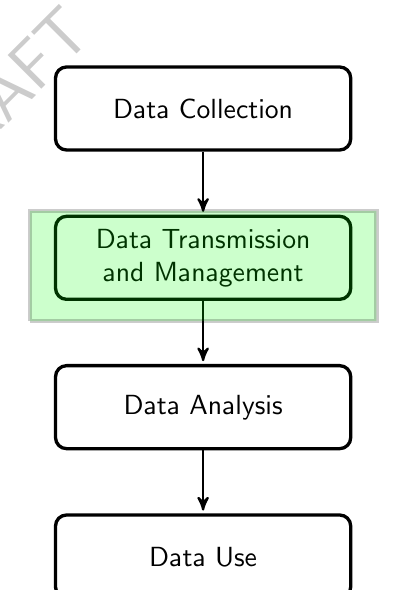
\begin{tikzpicture}[node distance=.8cm,  start chain=going below,]
     \node[punktchain, join] (DataCollection) {Data Collection};
     \node[punktchain, join] (DataManagement) {Data Transmission and Management};
     \node[punktchain, join] (DataAnalysis)   {Data Analysis};
     \node[punktchain, join] (DataUse) 		  {Data Use};
     \filldraw[ultra thick, draw=black, fill=green, opacity=0.2] (-2.2,-2.7) -- (-2.2,-1.3) -- (2.2,-1.3) -- (2.2,-2.7) -- (-2.2,-2.7) ;
\end{tikzpicture}
\end{minipage}
\begin{minipage}{.5\textwidth}
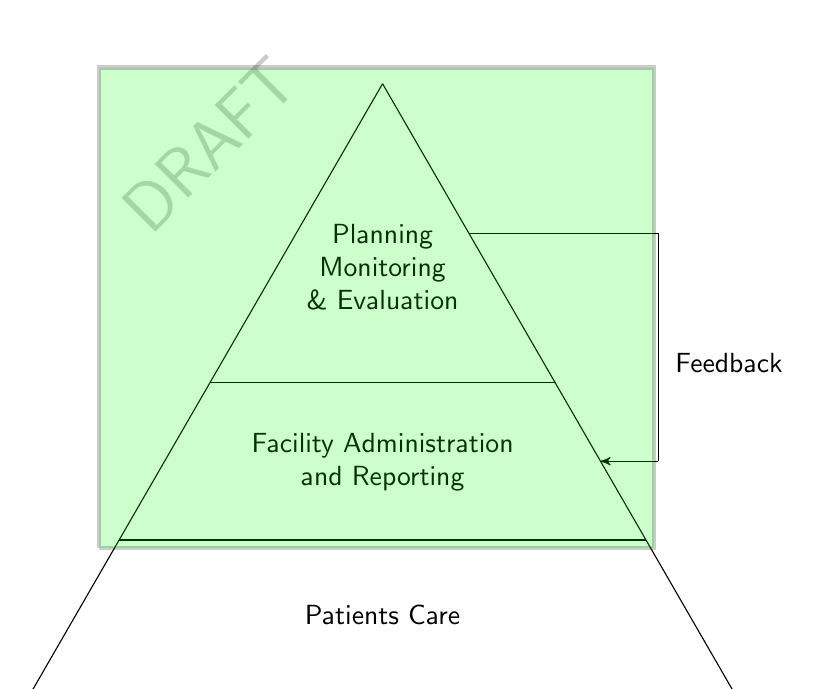
\begin{tikzpicture}[node distance=2cm]
\coordinate (A) at (-4.5,0) {};
\coordinate (B) at ( 4.5,0) {};
\coordinate (C) at ( 0,7.7942) {};
\draw[name path=AC] (A) -- (C);
\draw[name path=BC] (B) -- (C);
\draw (1.1,5.8971)--(3.5,5.8971) ;
\draw(3.5,5.8971)--(3.5,3) ;
\draw [->](3.5,3)--(2.77,3) ;
\node at (4.4,4.25) {Feedback};
\foreach \y/\A/\txtHigh in {0/Patients Care/0.8 ,2/Facility Administration \\ and Reporting/2.5,4/Planning \\ Monitoring \\ \& Evaluation /4.8}{
    \path[name path=horiz] (A|-0,\y) -- (B|-0,\y);
    \draw[name intersections={of=AC and horiz,by=P},
          name intersections={of=BC and horiz,by=Q}] (P) -- (Q)
          node[align = center,above] at (0,\txtHigh){\A};
          }
    \filldraw[ultra thick, draw=black, fill=green, opacity=0.2] (-3.6,1.9) -- (-3.6,8) -- (3.45,8) -- (3.45,1.9) -- (-3.6,1.9) ;
\end{tikzpicture}
\end{minipage}
\caption{Objective two definition}
\label{Paper Two}
\end{figure}

\subsection{Introduction to Interoperability work}

There are multiple reasons why interoperability between HMIS datasets is a great asset :
\begin{description}
\item[Comparison ] Being able to compare the results of different health systems is essential to be able to benchmark these results, or to make different systems benefit from each others' experiences.
\item[Validation / Completion] When multiple systems are operating in the same place, one can wish to compare results from different system in order to validate the data, or to fill missing data from another system.
\item[Co-analysis] Finally, pooling results from different systems provides higher power for analysis that can be made on different subjects.
\end{description}

It should be noted that the conditions for interoperability can be seen in different ways for each of these uses. If comparison of results necessitates that measured indicators have quasi identical definitions and methods, it is less the case for validation and completion, where a set of indicators can be used as a proxy to check the coherence or impute values of another data set. Finally, co-analysis may or may not require an exact mapping of indicators from different systems, depending of the subject matter.

There are multiple levels at which interoperability of data systems  has to be enforced \cite{braa_sahay_book}. At the Syntactic-Technical level, protocols have to be designed and implemented, to ensure that different data-systems can communicate. At the Organizational level, processes have to be implemented to allow the exchange and to define the condition of usage and aggregation of different data systems. Finally, at the Semantic level, qualitative meaning and understanding of the nature of the data being exchanged and compared has to be enforced.

%TODO Add graph on interoperaility from Saay Braa

I am interested in considering the semantic level of interoperability. Indeed, I will make the hypothesis that perfect standardization of HMIS indicators across contexts and platforms is an elusive goal, and may not even be desirable, as it is a factor of rigidity for HMIS, which should be able to evolve rapidly. I am thus be interested in defining methods to ensure ex-post semantic interoperability between different HMIS systems, in order to map indicators and with an objective of data validation and missing data imputation.

\subsection{Research questions}

This project is in the framework of a larger project, defining an interoperability framework between different systems. As part of this project, a tagging system has been defined that allows mapping of indicators from different standard hospital indicators sets. %% BIBLIO paper bluesquare

% TODO describe tagging system

Meanwhile, this tagging approach, if it is effective, has an important entry cost for users. Tagging a set of multiple dozens of indicators can indeed been an harrowing task in a field where quick fixes are the gold standard. %REF conceptual framework
We are thus working on two ways to improve this uptake. One is the definition of automatized learning methods that could help users in the tagging task. Another approach is to provide users with sufficiently strong incentives that the tagging work will be worth going through. As actors working towards interoperability of systems are likely to be middle tier actors in the information system, we think empowering them to use the benefits of interoperability for validation of data, correction of faulty data and completion of missing data would be a strong incentive.

I will thus explore methods to validate, correct and complete data sets from routine HMIS, and measure the benefits of indicators matching between different dataset to improve validation, correction and completion. This will be considered looking at different intermediary questions :

\begin{enumerate}
    \item What is a good metric to assert data quality and completeness of a given HMIS data set ?
    \item What is the performance of different approaches to HMIS data validation, correction and completion ?
    \item What is the benefit of using mapped datasets on this last metric ?
\end{enumerate}

Our main aim will be to gauge the credibility of a data value or a dataset.  Additionally, we want to provide some evidence as of what the source of error or missingness in a dataset is. There are three main situations we want to be able to differentiate between :
\begin{description}
\item[simple outlier] are situations when an isolated data value in a dataset is wrong, for one facility once. These are the situations that are the most commonly recognized as outliers.
\item[outlying report] are situations when all values of one report appear to be off. This may be due to an update in the tools or methods for some indicators, or to the training of a new Health Worker in the facility who does not fully comply with usual ways to compute indicators. To identify this type of issue, it is necessary to compare
\item[outlying facility] are situations when one facility is consistently reporting numbers that are different from surrounding facilities. This may happen when structural conditions in one facility are leading to discrepancies in data collection, or in data computation.
\end{description}

Our general approach will be to attach to each data value a probabilistic value for its credibility. The combination of these credibility measures for a dataset will give an overall estimation of the credibility of this dataset, and the type of error it may suffer from. In a third and last step, we will explore methods for imputation of data values with low credibility or for methods with low credibility.


\subsection{Data Validation / Method}

%% ie ce qu'on propose n'est pas orienté pour corriger les données mais pour construire un meilleurs système par la suite. Plus orienté développement et value l'utilisation des données plus que leur perfection. Imputation pour données fausses.

We will test two approaches to do so :

\begin{description}
\item[Error prediction] Using the validation dataset from OpenRBF, we will try and predict wrong data values using a simple predictive approach and bagging different Machine Learning Classification methods. Result of this approach will be a probabilistic assessment of data quality for each indicator value.
\item[Variable imputation] Using all available data, we will impute all data value and get a posterior estimated distribution of the value. The probability of the actual value in this posterior distribution will be taken as the probability of the value
\end{description}

\subsubsection{Error Prediction}

For a given indicator

\subsubsection{Variable Imputation}

For a given indicator $X_{i*}$ measured at time $t*$ in facility $f*$, we will compute an imputed distribution based on all other information available in our data.

$$ \widetilde{X}_{i^*,t^*,f^*} \sim \operatorname{D} \left(f\left(X_{i,t,f}\right)_{ \left(i,t,f\right) \neq \left(i^*,t^*,f*\right) } \right) $$

where $\operatorname{D}$ is an unspecified posterior distribution.

A distribution $\operatorname{P(\widetilde{X}_{i^*,t^*,f^*} )}$.

A threshold will be defined based on observed distributions.

We will test different approaches for this model.


\subsection{Credibility Pattern Screening}

The validity probability of each data value will be pooled at report, facility and district levels. An analysis of the distribution of credibility at each level of aggregation will be made to characterize the type of data error pattern in one of four categories : No error, Single outliers, Outlying report or Outlying facility.
\begin{description}
    \item[No error] will be situations in which no data values will be over the fixed threshold of acceptable credibility.
    \item[Single Outliers] will be situations in which less than 10\% of data values in a single report for a facility will be under the fixed threshold of acceptable credibility.
    \item[Outlying report] will be situations in which more than 10\% of data values in a single report for a given facility will be under the fixed threshold of acceptable credibility.
    \item[Outlying facilities] will be situations in which more than 10\% of data values will be under the fixed threshold of acceptable credibility in more than two consecutive reports for the same facility.
\end{description}

\subsection{Performance Metric}

Validation of these methods will be made using cross-validation. We will first evaluate the data validation framework independently of the indicators mapping framework. We will then test the performance of the combination of different indicator mapping methods and data validation methods.

\subsection{Data}

This work will be conducted in collaboration with the Belgian startup Bluesquare. Bluesquare has developed a data system for management and validation of Results Based Financing indicators, called OpenRBF. This solution has been implemented in Bénin in XX facilities in YY départements. Indicators are collected on a monthly basis in OpenRBF, and a data validation system is in place, to check the accuracy of reported indicators.

In the meantime Bénin has been implementing and using DHIS2 nationwide since AAAA. There is considerable interest in mapping indicators from the two systems, and using the two systems as validation and completion solutions.

%\subsection{Semantic interoperability framework}

%We will first test different approaches to semantic interoperability. This project is building on an existing project in which we have been defining and testing a structure tagging approach to interoperability. With this approach, each health service indicator in a given facility reporting framework is defined based on three dimensions : health issue, population target and type of service provided. A first level of testing has already implemented in Bénin, matching DHIS2 indicators with OpenRBF indicators. Using this simple method, it was possible to match correctly 15 of 21 indicators from the OpenRBF framework with a subset of 500 indicators from the DHIS2 framework.

%One of the biggest benefits of this approach is its ability to define a notion of \textit{distance} between indicators. Indicators that are related by one dimension will be farther apart from each other than indicators that are related by two dimensions. Also, for dimensions that are not defined on a discrete basis (for example age boundaries for a population), incomplete correspondence can be quantified. This notion of distance can in a later stage be used as a weight in comparison of different indicators. In the currently tested version, this distance is linearly additive, but other formulation of this distance can be tested.

%We will also test alternative approaches, such as Latent Semantic Indexing, and completely blind indicators matching based on values and trends.


\subsection{Timeline}

Figure \ref{Gantt2} will present a timeline for the realization of this objective.

\begin{figure}[h]
\begin{ganttchart}[vgrid,hgrid]{1}{24}
\gantttitle{2016}{12}
\gantttitle{2017}{12} \\
\gantttitlelist{1,...,12}{1} \gantttitlelist{1,...,12}{1}\\
%\ganttgroup{Group 1}{1}{7} \\
\ganttbar{Data Extraction}{1}{3} \\
\ganttbar{Data Cleaning}{2}{4} \\
\ganttbar{Data Analysis 1}{5}{6} \\
\ganttmilestone{Sharing First Results}{6} \\
\ganttbar{Data Analysis 2}{7}{9} \\
\ganttmilestone{Sharing Final Results}{9} \\
\ganttbar{Paper Writing}{9}{11} \\
\ganttmilestone{Paper Submission}{11}
\end{ganttchart}
\caption{Gantt Chart for Paper 2}
\label{Gantt2}
\end{figure}


\newpage
\section{Semantic approaches to HMIS interoperability for external data validation}

The second paper of this dissertation regards the management of data collected in hospitals in developing countries. The lack of standardization of indicators computed in different places or by different HMIS makes the use of HMIS data a complicated task. This issue is often handled as an issue of interoperability between systems.


\begin{figure}[ht]
	\begin{minipage}{.4\textwidth}
		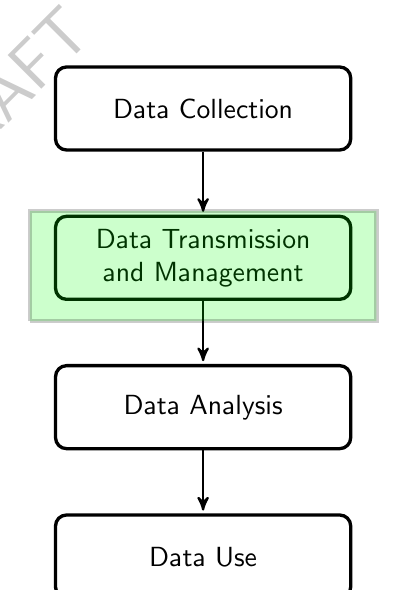
\begin{tikzpicture}[node distance=.8cm,  start chain=going below,]
			\node[punktchain, join] (DataCollection) {Data Collection};
			\node[punktchain, join] (DataManagement) {Data Transmission and Management};
			\node[punktchain, join] (DataAnalysis)   {Data Analysis};
			\node[punktchain, join] (DataUse) 		  {Data Use};
			\filldraw[ultra thick, draw=black, fill=green, opacity=0.2] (-2.2,-2.7) -- (-2.2,-1.3) -- (2.2,-1.3) -- (2.2,-2.7) -- (-2.2,-2.7) ;
		\end{tikzpicture}
	\end{minipage}
	\begin{minipage}{.5\textwidth}
		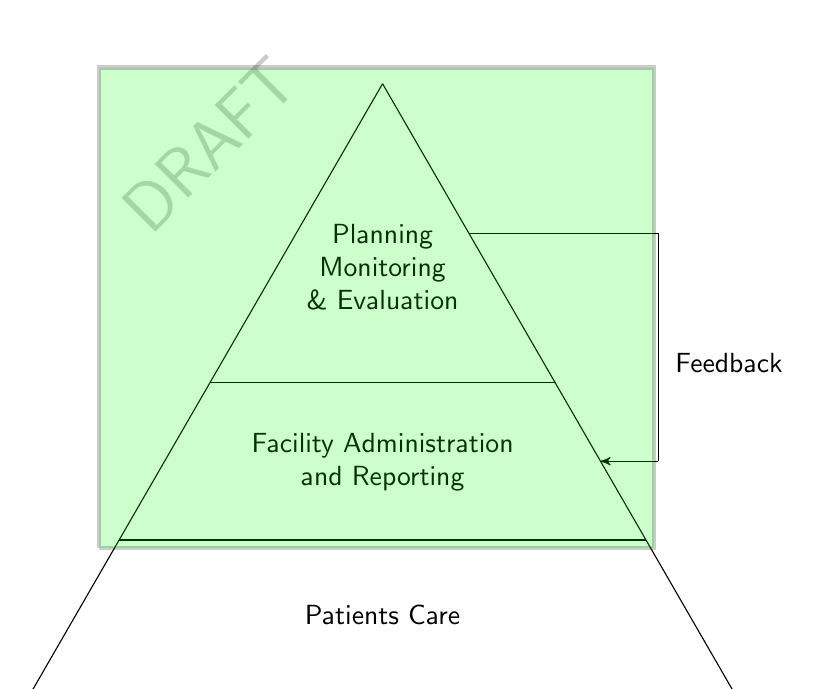
\begin{tikzpicture}[node distance=2cm]
			\coordinate (A) at (-4.5,0) {};
			\coordinate (B) at ( 4.5,0) {};
			\coordinate (C) at ( 0,7.7942) {};
			\draw[name path=AC] (A) -- (C);
			\draw[name path=BC] (B) -- (C);
			\draw (1.1,5.8971)--(3.5,5.8971) ;
			\draw(3.5,5.8971)--(3.5,3) ;
			\draw [->](3.5,3)--(2.77,3) ;
			\node at (4.4,4.25) {Feedback};
			\foreach \y/\A/\txtHigh in {0/Patients Care/0.8 ,2/Facility Administration \\ and Reporting/2.5,4/Planning \\ Monitoring \\ \& Evaluation /4.8}{
				\path[name path=horiz] (A|-0,\y) -- (B|-0,\y);
				\draw[name intersections={of=AC and horiz,by=P},
				name intersections={of=BC and horiz,by=Q}] (P) -- (Q)
				node[align = center,above] at (0,\txtHigh){\A};
			}
			\filldraw[ultra thick, draw=black, fill=green, opacity=0.2] (-3.6,1.9) -- (-3.6,8) -- (3.45,8) -- (3.45,1.9) -- (-3.6,1.9) ;
		\end{tikzpicture}
	\end{minipage}
	\caption{Objective two definition}
	\label{Paper Two}
\end{figure}

\subsection{Introduction to Interoperability work}

There are multiple reasons why  interoperability between HMIS datasets is a great asset :
\begin{description}
	\item[Comparison ] Being able to compare the results of different health systems is essential to be able to benchmark these results, or to make different systems benefit from each others' experiences.
	\item[Validation / Completion] When multiple systems are operating in the same place, one can wish to compare results from different system in order to validate the data, or to fill missing data from another system.
	\item[Co-analysis] Finally, pooling results from different systems provides higher power for analysis that can be made on different subjects.
\end{description}

It should be noted that the conditions for interoperability can be seen in different ways for each of these uses. If comparison of results necessitates that measured indicators have quasi identical definitions and methods, it is less the case for validation and completion, where a set of indicators can be used as a proxy to check the coherence or impute values of another data set. Finally, co-analysis may or may not require an exact mapping of indicators from different systems, depending of the subject matter.

There are multiple levels at which interoperability of data systems  has to be enforced \cite{braa_sahay_book}. At the Syntactic-Technical level, protocols have to be designed and implemented, to ensure that different data-systems can communicate. At the Organizational level, processes have to be implemented to allow the exchange and to define the condition of usage and aggregation of different data systems. Finally, at the Semantic level, qualitative meaning and understanding of the nature of the data being exchanged and compared has to be enforced.

%TODO Add graph on interoperaility from Saay Braa

I am interested in considering the semantic level of interoperability. Indeed, I will make the hypothesis that perfect standardization of HMIS indicators across contexts and platforms is an elusive goal, and may not even be desirable, as it is a factor of rigidity for HMIS, which should be able to evolve rapidly. I am thus be interested in defining methods to ensure ex-post semantic interoperability between different HMIS systems, in order to map indicators and with an objective of data validation and missing data imputation.

\subsection{Research questions}

This project is in the framework of a larger project, defining an interoperability framework between different systems. As part of this project, a tagging system has been defined that allows mapping of indicators from different standard hospital indicators sets. %% BIBLIO paper bluesquare

% TODO describe tagging system

Meanwhile, this tagging approach, if it is effective, has an important entry cost for users. Tagging a set of multiple dozens of indicators can indeed been an harrowing task in a field where quick fixes are the gold standard. %REF conceptual framework
We are thus working on two ways to improve this uptake. One is the definition of automatized learning methods that could help users in the tagging task. Another approach is to provide users with sufficiently strong incentives that the tagging work will be worth going through. As actors working towards interoperability of systems are likely to be middle tier actors in the information system, we think empowering them to use the benefits of interoperability for validation of data, correction of faulty data and completion of missing data would be a strong incentive.

I will thus explore methods to validate, correct and complete data sets from routine HMIS, and measure the benefits of indicators matching between different dataset to improve validation, correction and completion. This will be considered looking at different intermediary questions :

\begin{enumerate}
	\item What is a good metric to assert data quality and completeness of a given HMIS data set ?
	\item What is the performance of different approaches to HMIS data validation, correction and completion ?
	\item What is the benefit of using mapped datasets on this last metric ?
\end{enumerate}

Our main aim will be to gauge the credibility of a data value or a dataset.  Additionally, we want to provide some evidence as of what the source of error or missingness in a dataset is. There are three main situations we want to be able to differentiate between :
\begin{description}
	\item[simple outlier] are situations when an isolated data value in a dataset is wrong, for one facility once. These are the situations that are the most commonly recognized as outliers.
	\item[outlying report] are situations when all values of one report appear to be off. This may be due to an update in the tools or methods for some indicators, or to the training of a new Health Worker in the facility who does not fully comply with usual ways to compute indicators. To identify this type of issue, it is necessary to compare
	\item[outlying facility] are situations when one facility is consistently reporting numbers that are different from surrounding facilities. This may happen when structural conditions in one facility are leading to discrepancies in data collection, or in data computation.
\end{description}

Our general approach will be to attach to each data value a probabilistic value for its credibility. The combination of these credibility measures for a dataset will give an overall estimation of the credibility of this dataset, and the type of error it may suffer from. In a third and last step, we will explore methods for imputation of data values with low credibility or for methods with low credibility.


\subsection{Data Validation / Method}

%% ie ce qu'on propose n'est pas orienté pour corriger les données mais pour construire un meilleurs système par la suite. Plus orienté développement et value l'utilisation des données plus que leur perfection. Imputation pour données fausses.

We will test two approaches to do so :

\begin{description}
	\item[Error prediction] Using the validation dataset from OpenRBF, we will try and predict wrong data values using a simple predictive approach and bagging different Machine Learning Classification methods. Result of this approach will be a probabilistic assessment of data quality for each indicator value.
	\item[Variable imputation] Using all available data, we will impute all data value and get a posterior estimated distribution of the value.
\end{description}

\subsubsection{Error Prediction}

For a each indicator value, we will model the probability that the value is right. We will use a logistic model specified as :
%% TODO specification logistic model

Using \textit{Forward model selection} and training models on data on verified values (cf. \ref{paper2_data}), we will find the best models to predict data value errors. We will then use this model out of sample to compute the probability a value is true on each value.

\subsubsection{Variable Imputation}

For a given indicator $X_{i*}$ measured at time $t*$ in facility $f*$, we will compute an imputed distribution based on all other information available in our data. A general representation of this approach could be written as:

$$ \widetilde{X}_{i^*,t^*,f^*} \sim \operatorname{D} \left(f\left(X_{i,t,f}\right)_{ \left(i,t,f\right) \neq \left(i^*,t^*,f*\right) } \right) $$

where $\operatorname{D}$ is an unspecified distribution derived from a function of all available data excluding the data point $\widetilde{X}_{i^*,t^*,f^*}$.

Using verified data as our validation set, we will define a threshold for credibility of data that we will later use as a decision rule for considering data as regular or outlying (see \ref{paper2_credib_pattern}).

We will test different approaches for this model.
% TODO Document different models I will use


\subsection{Credibility Pattern Screening}
\label{paper2_credib_pattern}

The validity probability of each data value will be pooled at report, facility and district levels. An analysis of the distribution of credibility at each level of aggregation will be made to characterize the type of data error pattern in one of four categories : No error, Single outliers, Outlying report or Outlying facility.
\begin{description}
	\item[No error] will be situations in which no data values will be over the fixed threshold of acceptable credibility.
	\item[Single Outliers] will be situations in which less than 10\% of data values in a single report for a facility will be under the fixed threshold of acceptable credibility.
	\item[Outlying report] will be situations in which more than 10\% of data values in a single report for a given facility will be under the fixed threshold of acceptable credibility.
	\item[Outlying facilities] will be situations in which more than 10\% of data values will be under the fixed threshold of acceptable credibility in more than two consecutive reports for the same facility.
\end{description}

\subsection{Performance Metric}

Validation of these methods will be made using cross-validation. We will first evaluate the data validation framework independently of the indicators mapping framework. We will then test the performance of the combination of different indicator mapping methods and data validation methods.

\subsection{Data}
\label{paper2_data}

This work will be conducted in collaboration with the Belgian startup Bluesquare. Bluesquare has developed a data system for management and validation of Results Based Financing indicators, called OpenRBF. This solution has been implemented in Bénin in XX facilities in YY départements. Indicators are collected on a monthly basis in OpenRBF, and a data validation system is in place, to check the accuracy of reported indicators.

In the meantime Bénin has been implementing and using DHIS2 nationwide since AAAA. There is considerable interest in mapping indicators from the two systems, and using the two systems as validation and completion solutions.

%\subsection{Semantic interoperability framework}

%We will first test different approaches to semantic interoperability. This project is building on an existing project in which we have been defining and testing a structure tagging approach to interoperability. With this approach, each health service indicator in a given facility reporting framework is defined based on three dimensions : health issue, population target and type of service provided. A first level of testing has already implemented in Bénin, matching DHIS2 indicators with OpenRBF indicators. Using this simple method, it was possible to match correctly 15 of 21 indicators from the OpenRBF framework with a subset of 500 indicators from the DHIS2 framework.

%One of the biggest benefits of this approach is its ability to define a notion of \textit{distance} between indicators. Indicators that are related by one dimension will be farther apart from each other than indicators that are related by two dimensions. Also, for dimensions that are not defined on a discrete basis (for example age boundaries for a population), incomplete correspondence can be quantified. This notion of distance can in a later stage be used as a weight in comparison of different indicators. In the currently tested version, this distance is linearly additive, but other formulation of this distance can be tested.

%We will also test alternative approaches, such as Latent Semantic Indexing, and completely blind indicators matching based on values and trends.


\subsection{Timeline}

Figure \ref{Gantt2} will present a timeline for the realization of this objective.

\begin{figure}[h]
	\begin{ganttchart}[vgrid,hgrid]{1}{24}
		\gantttitle{2016}{12}
		\gantttitle{2017}{12} \\
		\gantttitlelist{1,...,12}{1} \gantttitlelist{1,...,12}{1}\\
		%\ganttgroup{Group 1}{1}{7} \\
		\ganttbar{Data Extraction}{1}{3} \\
		\ganttbar{Data Cleaning}{2}{4} \\
		\ganttbar{Data Analysis 1}{5}{6} \\
		\ganttmilestone{Sharing First Results}{6} \\
		\ganttbar{Data Analysis 2}{7}{9} \\
		\ganttmilestone{Sharing Final Results}{9} \\
		\ganttbar{Paper Writing}{9}{11} \\
		\ganttmilestone{Paper Submission}{11}
	\end{ganttchart}
	\caption{Gantt Chart for Paper 2}
	\label{Gantt2}
\end{figure}


\newpage
\section{Data Use}

construction d'un espace politique d'équivalence et de codage


"Les outils statistiques permettent de découvrir ou de créer des êtres sur lesquels prendre appui pour décrire le monde et agir sur lui"

\subsection{Information in Health Systems}

%BIBLIO chaperon88 le PMSI est arrivé après au mois 4 échecs de systèmes d'information sur la morbidité hospitalière (45;49;53;70). Sa spécificté est de lier le déboursement des apports financiers. Systèmes précédents avaient pb avec le risque de controle 1958 reform of hospital morbidity collection forms from methods at Hotel Dieu : elle va tres rapidement echouert: le questionnaire demande un sercroît de travail aux services administratifs confrontés dans le même temps à une nomrlasation de l'ensemble des imprimiés : côté médical l'investigation est ressentie comme un contrôle de l'administration sur l'activité médicale. (FROM RAZPPORT ECOLE DES MINES)



\begin{figure}[ht]
\begin{minipage}{.4\textwidth}
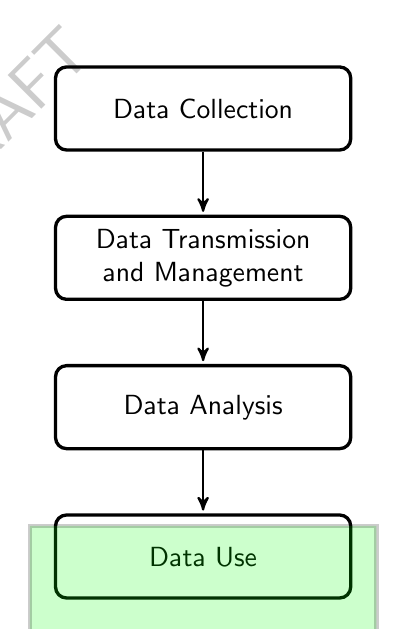
\begin{tikzpicture}[node distance=.8cm,  start chain=going below,]
     \node[punktchain, join] (DataCollection) {Data Collection};
     \node[punktchain, join] (DataManagement) {Data Transmission and Management};
     \node[punktchain, join] (DataAnalysis)   {Data Analysis};
     \node[punktchain, join] (DataUse) 		  {Data Use};
     \filldraw[ultra thick, draw=black, fill=green, opacity=0.2] (-2.2,-6.7) -- (-2.2,-5.3) -- (2.2,-5.3) -- (2.2,-6.7) -- (-2.2,-6.7) ;
\end{tikzpicture}
\end{minipage}
\begin{minipage}{.5\textwidth}
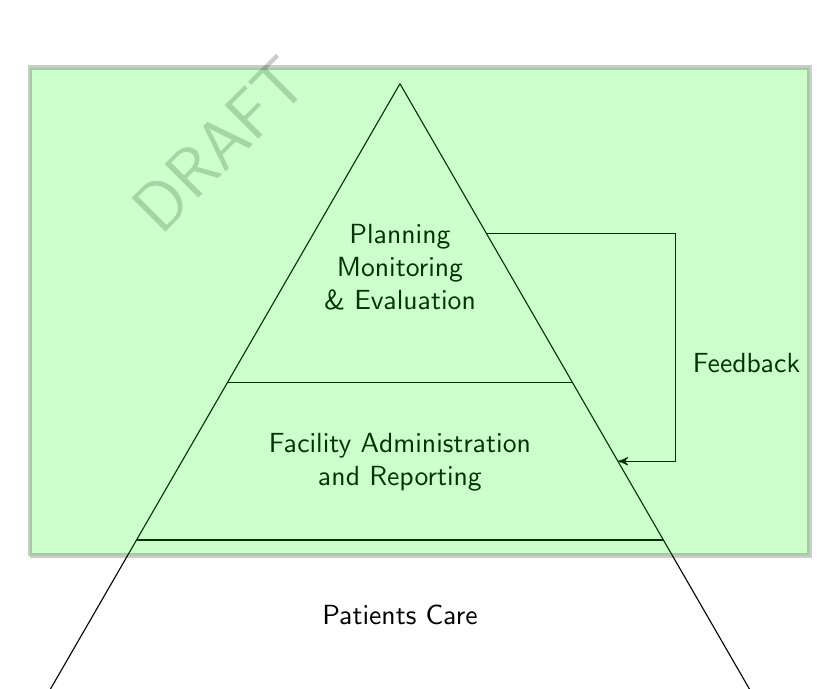
\begin{tikzpicture}[node distance=2cm]
\coordinate (A) at (-4.5,0) {};
\coordinate (B) at ( 4.5,0) {};
\coordinate (C) at ( 0,7.7942) {};
\draw[name path=AC] (A) -- (C);
\draw[name path=BC] (B) -- (C);
\draw (1.1,5.8971)--(3.5,5.8971) ;
\draw(3.5,5.8971)--(3.5,3) ;
\draw [->](3.5,3)--(2.77,3) ;
\node at (4.4,4.25) {Feedback};
\foreach \y/\A/\txtHigh in {0/Patients Care/0.8 ,2/Facility Administration \\ and Reporting/2.5,4/Planning \\ Monitoring \\ \& Evaluation /4.8}{
    \path[name path=horiz] (A|-0,\y) -- (B|-0,\y);
    \draw[name intersections={of=AC and horiz,by=P},
          name intersections={of=BC and horiz,by=Q}] (P) -- (Q)
          node[align = center,above] at (0,\txtHigh){\A};
          }
    \filldraw[ultra thick, draw=black, fill=green, opacity=0.2] (-4.7,1.8) -- (-4.7,8) -- (5.2,8) -- (5.2,1.8) -- (-4.7,1.8) ;
\end{tikzpicture}
\end{minipage}
\caption{Objective four definition}
\label{Paper Four}
\end{figure}

The use of statistical information for the management of complex organizations has evolved since the beginning of the XIXth century. Since the invention of population by XVIIIth century demographers[DESROSIERES], and the integration of numbers in the political and administrative language in the second XIXth century [PORTER], multiple types of information have been used for the orientation of public policies and the administration of public services. Meanwhile, the rise of epidemiology and the critalization of a body of knowledge around the institutions in charge of the defense of Public Health helped creating a specific Public Health oriented spin on quantitative information for health systems.

The use of data for policy making is a combination of data sources, statistical methods, and political or social norms, that will define the conditions of utilisation of statistical evidence for policy making. Finding the proper data source, being able to analyze it and incorporating the results of this analysis in a political process is essential to the proper use and utilization of information systems. In this regard, Alain Desrosières has shown how two traditions have been cohabiting in the early ages of the production of social statistics\cite{admin_savant}.

%In Global Health, the use of data for the definition of \textit{evidence based} intervention and policies has emerged as a panacea for project design and management. There are nonetheless difficulties in this regard. The global nature of public health means that statistical data available for analysis is by nature scattered and varied.

%reductio ad M\&E

\begin{quote}
The first tradition is administrative, and is based on political science and the law, on the German Staatenkunde, from the time of Conring and Achenwall. It is more taxonomic than metrological: it is designed to classify facts systematically rather than measure them, which is the essence of the other tradition, the "English" tradition. The latter, inspired more by the natural sciences and by progress made in measurement and probability theories, is a distant relation of the English political arithmetic of Graunt and Petty.
\end{quote}

Desrosières later shows how these two traditions have bee reconciled in the modern figure of the statistician, at the same time administrator and scientist. It is useful to keep considering this tension when thinking about maturing statistical systems like HMIS. Being able to distinguish between situations when actors of HMIS are acting as administrators, and when the position is that of a metrician is essential to understand HMIS issues and offer informed solutions.

This distinction is essential at many levels. The whole debate around the level of uncertainty that is bearable around a measurement is not only important for statisticians. Choosing a given approach will have an impact on how primary data will be collected, how it will be analyzed, and how it will be used. In many usages of HMIS, complete enumeration is deemed necessary, but this can be discussed. What is the level of confidence one can bear around the estimation of a stock of drugs ?

In sub-Saharan Africa, this tension is reinforced by a political tradition that has been structured around the colonial state. The structures and political traditions coming from this specific have complex relationships with the notions of uncertainty and control. Moreover, these structure are reenacting the colonial culture of exogeneous power structure, through that international actors take in the governance of African country.

This last paper will aim at understanding how some program managers in Mali the data available in HMIS, and how it impacts the way they think, design and implement HMIS programs. We will interrogate the notions of uncertainty, sampling, control and norms for this managers, and their appreciation and use of numerical evidence.

UNFINISHED

Reflections on social conditions of HMIS data usage  / politics of administrative statistics.

Data is not produced to create knowledge, but to implement disciplinary monitoring. Thinking mainly in terms of indicators.


    Figure \ref{Gantt4} will present a timeline for the realization of this objective.

    \begin{figure}[h]
    \begin{ganttchart}[vgrid,hgrid]{1}{24}
    \gantttitle{2016}{12}
    \gantttitle{2017}{12} \\
    \gantttitlelist{1,...,12}{1} \gantttitlelist{1,...,12}{1}\\
    %\ganttgroup{Group 1}{1}{7} \\
    \ganttbar{Data Extraction}{1}{3} \\
    \ganttbar{Data Cleaning}{2}{4} \\
    \ganttbar{Data Analysis 1}{5}{6} \\
    \ganttmilestone{Sharing First Results}{6} \\
    \ganttbar{Data Analysis 2}{7}{9} \\
    \ganttmilestone{Sharing Final Results}{9} \\
    \ganttbar{Paper Writing}{9}{11} \\
    \ganttmilestone{Paper Submission}{11}
    \end{ganttchart}
    \caption{Gantt Chart for Paper 4}
    \label{Gantt4}
    \end{figure}



%%%%%%%%%%%%%%%%%%%%%%%%%%%%%%%%%%%%%%%%%%%%%%%%%%%
%% 			BIBLIOGRAPHY
%%%%%%%%%%%%%%%%%%%%%%%%%%%%%%%%%%%%%%%%%%%%%%%%%%%
%\cleardoublepage
%\phantomsection\addcontentsline{toc}{section}{Références}
\newpage
\bibliography{bibliographie}


\end{document}
